\section{Methods}

\begin{figure*}[t]
\centering
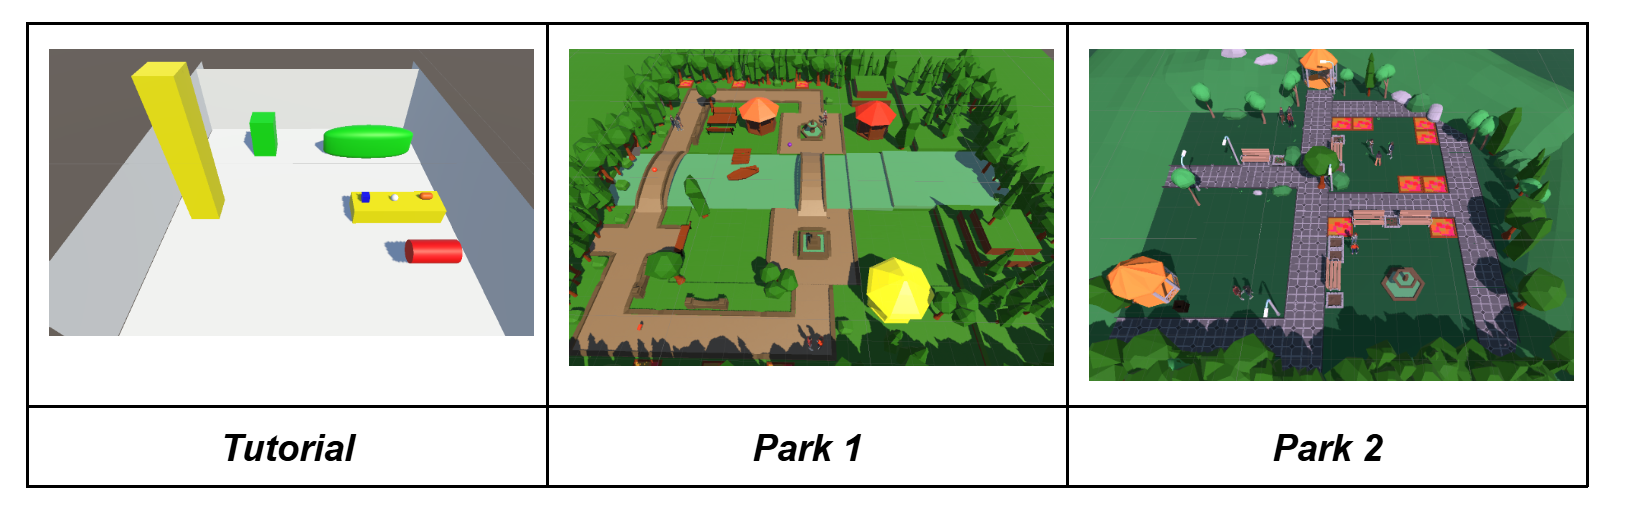
\includegraphics[width=350pt]{virtual_environments.png}
\caption{\label{fig: Virtual Environments} The three virtual environments used in the study. From left to right, the Tutorial contains various simplistic 3D objects such as yellow and green cubes, Park 1 contains a large river and several colorful gazebos, and Park 2 contains colorful flower beds and a series of benches for resting throughout the park.}
    \Description{A table with three images of the virtual environments used in the study. On the far left is an image of the tutorial room, a simple white room with various geometrical shapes, including a yellow, horizontal cube acting as a table with three interactable shapes resting on it. In the middle is a screenshot of the first park with trees scattered about and a river cutting through, populated by stone walkways and bridges, two water fountains, three gazebos, and three groups of avatars. On the right is a screenshot of the second park, a brightly-lit park with stone tile walkways around a few square patches of grass, two gazebos, and a group of avatars gathered for a dance party.
}
\end{figure*}

We refined the AI guide prototype from our previous design \cite{collins2024ai}, implementing specific changes (such as specific personas and re-engineered prompts) to study its use. We recruited BLV participants and observed them performing individual and social tasks in virtual environments using the guide. Finally, we conducted interviews about participants’ VR experience.

\subsection{Participants}

We recruited 16 participants (see Table \ref{tab: Participants}) through a partner organization, the LightHouse for the Blind and Visually Impaired in San Francisco, which provides services to BLV individuals. Participants were eligible for our study if they identified as blind or low vision, were at least 18 years old, could travel for an in-person study, and met the Meta Quest Health and Safety Guidelines \cite{guidelines}. Each participant was compensated \$100. Participants’ ages ranged from 22 to 75 (SD = 14.23, 7 women, 9 men). Eight participants identified as low vision and eight as blind. All procedures were approved by our university’s Institutional Review Board.

\begin{table*}[h!]
    \footnotesize 
    \centering
    \caption{\label{tab: Participants} Participant demographics. F = female, M = male. Participant information is self-reported. NR indicates that participants chose not to report that information.} 
    \begin{tabular}{p{1.4cm}p{0.3cm}p{1.0cm}p{2.0cm}p{1.5cm}p{2.0cm}p{2.0cm}p{4.0cm}}
    \toprule
      \textbf{Pseudonym}&  \textbf{Age}&  \textbf{Gender}&  \textbf{Visual Condition}&  \textbf{Etiology}&  \textbf{Visual Acuity}&   \textbf{Visual Field}&  \textbf{Navigation Tools Used} \\
     \midrule 
    
   \textbf{Niya}&   45&   F&  Blind; No Light Perception&  NR&    NR&     NR&  White Cane; Human Guide; Navigation Apps; Tactile Maps\\ 
    \midrule
    
    \textbf{Anika}&   46& F&  Low Vision&   Optic Atrophy&    R: 20/400, L: 20/200&     Vision in upper field of left eye, right eye blurry&  White Cane; Navigation Apps\\ 
    \midrule

     \textbf{Teo} & 51 & M&  Low Vision&   Cortical Impairment&    R: 20/400, L: 20/400&     NR&  White Cane; Navigation Apps; GPS Devices\\ 
    \midrule
    
      \textbf{Nikolai}&    34&    M& Partially Sighted; Legally Blind; Night Blindness; Central Vision Loss&   NR&    NR&     NR&  Navigation Apps\\ 
    \midrule
    
      \textbf{Sara}&    22& F&    Legally Blind&     Dual Optic Coloboma&    NR&     NR&  White Cane; Navigation Apps\\ 
    \midrule

      \textbf{Xiran}&    38& F&    Legally Blind; Night Blindness; Peripheral Vision Loss &    NR&    NR&     NR&  White Cane; Human Guide; Navigation Apps\\ 
    \midrule
    
      \textbf{Yuki}&    37& M&    Blind; No Light Perception&     NR&    NR&     NR&  White Cane; Navigation Apps\\ 
    \midrule
    
      \textbf{Maritza}&    75& F&   Blind; No Light Perception&     NR&    NR&     NR&  White Cane; Guide Dog; Human Guide; Navigation Apps; GPS Devices\\ 
    \midrule
    
      \textbf{Aiden}&    45& M&   Blind; Light Perception Only; Legally Blind&     NR&    NR&     No vision in left eye, light detection in right eye&  White Cane; Human Guide; Navigation Apps; GPS Devices\\ 
    \midrule
    
      \textbf{Len}&    29& M&  Low Vision; Legally Blind; Night Blindness; Peripheral Vision Loss&    Retinitis Pigmentosa&    NR&     NR&  White Cane; Human Guide; Navigation Apps\\ 
    \midrule
    
      \textbf{Siobhan}&    55& F&  Blind; No Light Perception&   Retinopathy of Prematurity&    NR&     NR&  White Cane; Guide Dog; Navigation Apps; Tactile Maps; GPS Devices; AR Glasses\\ 
    \midrule
    
      \textbf{Isaiah}&    54& M&  Partially Sighted&    NR&    R: 20/200, L: 20/150&     NR&  White Cane; Human Guide; Navigation Apps\\ 
    \midrule
    
      \textbf{Li}&    55& M&  Low Vision; Legally Blind; Peripheral Vision Loss&    Diabetic Retinopathy&    NR&     NR&  White Cane; Human Guide; Navigation Apps\\ 
    \midrule

      \textbf{Jamal}&    67& M&  Low Vision&    NR&    R: None, L: 20/200&     No vision in right eye, minimal field in left eye&  Navigation Apps\\ 
    \midrule

      \textbf{Yadriel}&    27& M&  Low Vision; Color Blindness&    Autosomal Optic Atrophy&    R: 20/300, L: 20/400&     Normal visual field&  Do not use any\\ 
    \midrule

      \textbf{Jiwoo}&    28& M&  Low Vision; Partially Sighted; Legally Blind; Color Blindness&    NR&    NR&     NR&  Navigation Apps\\ 
    
     \bottomrule
    \end{tabular}
    \Description{Information about our participant demographics. Contains all textual content.}
\end{table*}

\subsection{Procedure} \label{sec: Procedure}

We conducted a single, 90-minute study session with each participant at a conference room provided by LightHouse. Each session comprised three parts: a VR tutorial, two rounds of VR tasks, and a semi-structured interview. During the VR tutorial, participants explored the AI guide’s features in its human persona. Participants then completed the VR tasks using the dog and the robot personas (see section \ref{sec: Prototype Design and Implementation} for explanation of personas). These tasks were counterbalanced so that each participant experienced both personas as well as different environments (see Table \ref{tab: Counterbalancing Procedures} for detailed counterbalancing and study procedures).

\begin{table*}[htbp]
\centering
\caption{\label{tab: Counterbalancing Procedures}The counterbalanced study conditions (e.g., duration, park, persona) across all groups of participants. Group 1 = Niya, Anika, Teo, Nikolai; Group 2 = Sara, Xiran, Yuki, Maritza; Group 3 = Aiden, Len, Siobhan, Isaiah; Group 4 = Li, Jamal, Yadriel, Jiwoo. Participants completed two tasks per study phase (i.e., one individual and one social task).}
\label{tab:study_conditions}
\setlength{\tabcolsep}{5pt} % Adjust column separation for better fit
\begin{tabular}{cccccc}
\toprule
\textbf{Group} & \textbf{Phase} & \textbf{Task Type} & \textbf{Duration} & \textbf{Park} & \textbf{Persona} \\
\textbf{(N = 4 participants per group)} & & & & \textbf{Assignment} & \textbf{Assignment} \\
\midrule
\multirow{4}{*}{\textbf{1}} & \multirow{2}{*}{Round 1} & Individual Task (Exploration) & 10 minutes & \multirow{2}{*}{Park 1} & \multirow{2}{*}{Dog} \\
 & & Social Task (Tour) & 15 minutes & & \\
\cmidrule{2-6}
 & \multirow{2}{*}{Round 2} & Individual Task (Exploration) & 10 minutes & \multirow{2}{*}{Park 2} & \multirow{2}{*}{Robot} \\
 & & Social Task (Tour) & 15 minutes & & \\
\midrule
\multirow{4}{*}{\textbf{2}} & \multirow{2}{*}{Round 1} & Individual Task (Exploration) & 10 minutes & \multirow{2}{*}{Park 1} & \multirow{2}{*}{Dog} \\
 & & Social Task (Tour) & 15 minutes & & \\
\cmidrule{2-6}
 & \multirow{2}{*}{Round 2} & Individual Task (Exploration) & 10 minutes & \multirow{2}{*}{Park 2} & \multirow{2}{*}{Robot} \\
 & & Social Task (Tour) & 15 minutes & & \\
\midrule
\multirow{4}{*}{\textbf{3}} & \multirow{2}{*}{Round 1} & Individual Task (Exploration) & 10 minutes & \multirow{2}{*}{Park 1} & \multirow{2}{*}{Robot} \\
 & & Social Task (Tour) & 15 minutes & & \\
\cmidrule{2-6}
 & \multirow{2}{*}{Round 2} & Individual Task (Exploration) & 10 minutes & \multirow{2}{*}{Park 2} & \multirow{2}{*}{Dog} \\
 & & Social Task (Tour) & 15 minutes & & \\
\midrule
\multirow{4}{*}{\textbf{4}} & \multirow{2}{*}{Round 1} & Individual Task (Exploration) & 10 minutes & \multirow{2}{*}{Park 1} & \multirow{2}{*}{Robot} \\
 & & Social Task (Tour) & 15 minutes & & \\
\cmidrule{2-6}
 & \multirow{2}{*}{Round 2} & Individual Task (Exploration) & 10 minutes & \multirow{2}{*}{Park 2} & \multirow{2}{*}{Dog} \\
 & & Social Task (Tour) & 15 minutes & & \\
\bottomrule
\end{tabular}
\end{table*}

The tutorial began in a simple square room filled with primitive 3D objects. This introduction allowed participants to become familiar with the VR platform and the AI guide controls. Participants learned to move around the room, pick up objects, and call their guide. The tutorial concluded once participants felt comfortable with these basic interactions.

Participants then proceeded to the first of two VR tasks: exploring a virtual park with the AI guide. The goal of this task was to observe use of a guide in \textit{individual} settings. Participants were placed in one of two virtual environments modeled after parks from our study on human guides (see section \ref{sec: Prototype Design and Implementation}) \cite{collins2023guide}. Participants were asked to familiarize themselves with key landmarks (e.g., gazebos, a river). This task ended after ten minutes or once the participant indicated they were comfortable with the park contents.

The second task required participants to give a tour of the same park to two joining researchers acting as confederates. This task was designed to observe guide use in \textit{social} settings, where participants had to balance their use of the guide with social interaction. Participants were instructed to answer any questions from the confederates and lead them to at least two park landmarks. This task concluded after fifteen minutes or once they had completed the tour. Participants then repeated both tasks in a different park with a new guide persona.

Throughout the entire study, confederates used human avatars matching their preferred gender. To standardize confederate behavior, senior researchers on the team developed behavioral guidelines (included in supplementary materials). For example, the guidelines instructed confederates to pretend to be sighted participants of a different study who were unfamiliar with the guide. We implemented this to avoid influencing participants’ guide usage if they believed the confederates were experienced with it. In addition, the guidelines provided examples of questions and topics to discuss (e.g., the guide, the parks, hobbies) to ensure natural interaction. They also included instructions for movement throughout the study, such as pre-determined rendezvous points with participants, best practices for following participants, and examples of natural body language or gestures to use.

%\begin{figure*}[t]
\centering
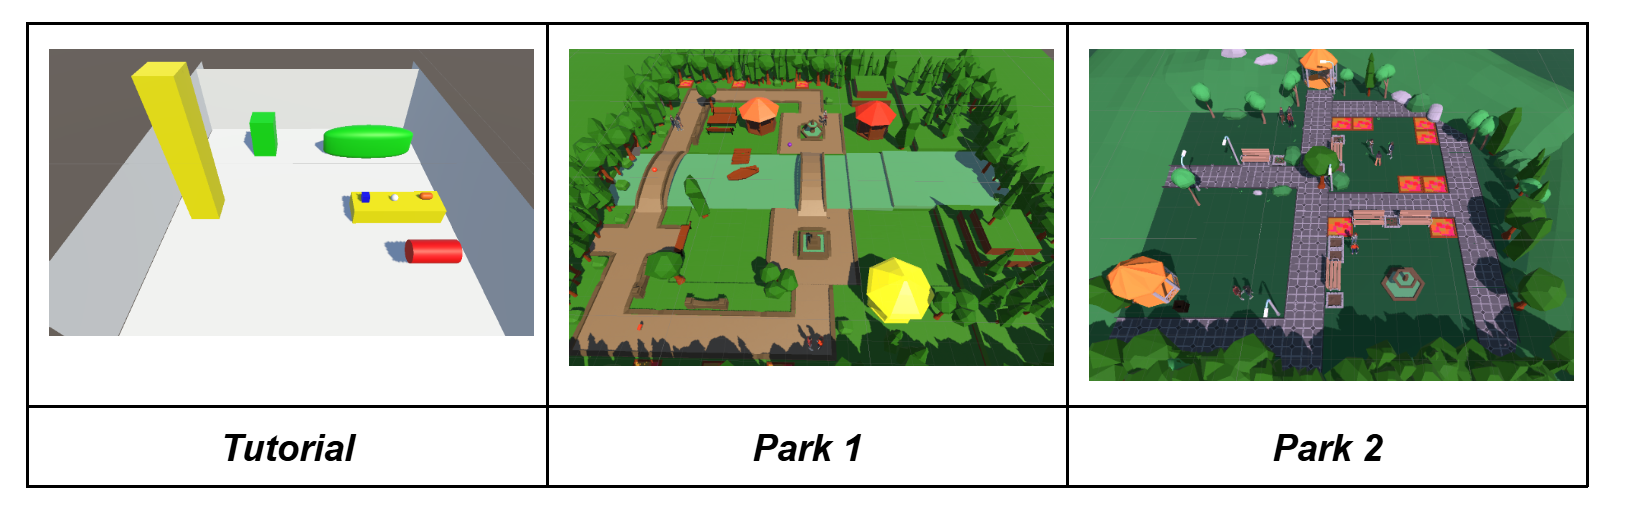
\includegraphics[width=350pt]{virtual_environments.png}
\caption{\label{fig: Virtual Environments} The three virtual environments used in the study. From left to right, the Tutorial contains various simplistic 3D objects such as yellow and green cubes, Park 1 contains a large river and several colorful gazebos, and Park 2 contains colorful flower beds and a series of benches for resting throughout the park.}
    \Description{A table with three images of the virtual environments used in the study. On the far left is an image of the tutorial room, a simple white room with various geometrical shapes, including a yellow, horizontal cube acting as a table with three interactable shapes resting on it. In the middle is a screenshot of the first park with trees scattered about and a river cutting through, populated by stone walkways and bridges, two water fountains, three gazebos, and three groups of avatars. On the right is a screenshot of the second park, a brightly-lit park with stone tile walkways around a few square patches of grass, two gazebos, and a group of avatars gathered for a dance party.
}
\end{figure*}

We concluded our study with a 30-minute semi-structured interview. Participants responded to Likert-scale statements (rated 1 to 5; see Figure \ref{fig: Likert Guide Ratings}) and answered open-ended questions across nine categories: usability, usefulness, joy of use, social comfort, scene understanding, object perception, navigation, appearance, and areas for improvement. Example questions included:

\begin{itemize}
	\item \textbf{“Which of the guide personas did you prefer using? Why?”}
	\item \textbf{“Were there any tasks you felt the guide struggled to assist you with?”}
	\item \textbf{“How effective were the guide’s descriptions of the scenes you were in?”}
\item \textbf{“How do you believe the guide impacted others’ perceptions of you?”}
\end{itemize}

\subsection{Prototype Design and Implementation} \label{sec: Prototype Design and Implementation}

We refined our original design of an AI guide \cite{collins2024ai}, incorporating specific changes informed by pilot studies in our current work.

Our refined AI guide offered three primary capabilities of the original guide: (1) providing \textbf{visual descriptions} of the environment, (2) assisting users in \textbf{moving their avatars} to specified locations or objects upon request, and (3) placing spatialized \textbf{audio beacons} on objects to aid in orientation. Users could activate or mute the guide using the secondary buttons on their VR controllers. They interacted with the guide via specific (e.g. “Take me to the Northern Fountain”) or vague (e.g., “What is this bluish-gray blob in front of me?”) voice commands.

\begin{table*}[t]
            \small
            \renewcommand{\arraystretch}{1.7}
            \begin{center}
            \caption{\label{tab: Guide Personas} Our guide’s three personas: the human, the guide dog, and the robot. The voices mentioned for each persona (Alloy, Nova, and Onyx) are OpenAI’s default TTS voices \cite{openai-tts}. Audio samples of each voice can be found at the cited link. The personality prompts were sent to GPT-4 to shape the guide's responses (see supplemental materials). All columns are based on our previous designs from Collins et al. \cite{collins2024ai}, except for Speech Sample, which was produced by our current implementation of the AI guide.}
                \begin{tabular}{|P{1cm} | M{2cm} | P{2cm} | P{2cm} | P{2cm} | P{2cm} |P{3.2cm} |}
                    \hline
                    \textbf{Persona} & \textbf{Guide Avatar} & \textbf{Guide Description} &
                    \textbf{Guide Movement} &
                    \textbf{Voice + Speech Characteristics} &
                    \textbf{Personality Prompt} & \textbf{Speech Sample} \\ \hline
                    \textbf{Human} & \raisebox{-\totalheight}{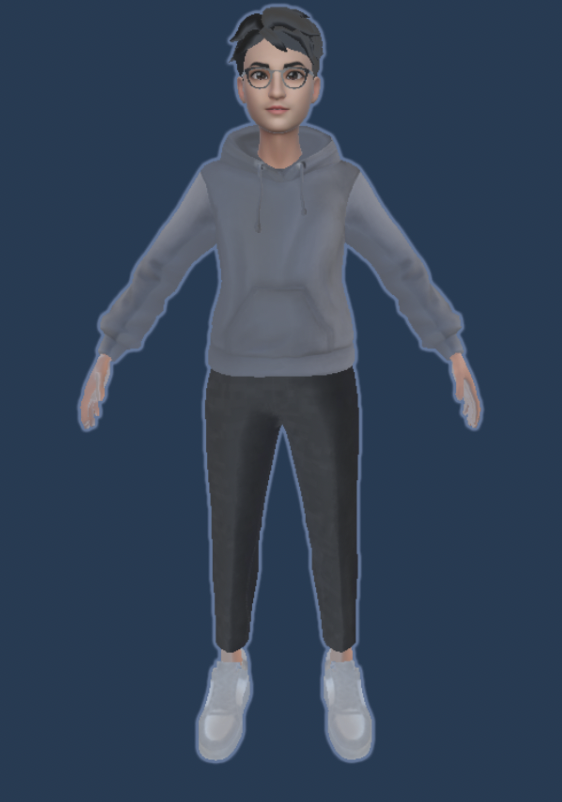
\includegraphics[width=1.8cm, height=2.3cm]{human_guide.png}} & An androgynous human with short black hair and glasses, wearing a gray hoodie and black pants. & Follows behind the user from an arm’s length away. Footstep sound effects indicate movement. & \textit{Alloy,} androgynous voice, medium formality (some jokes, casual speech), averages 101.2 words per response & Warm, friendly, but still professional sighted guide & \textit{The scene around you is a simple, geometric landscape composed of distinctive objects. To your right stands the Tall Building, a towering yellow cube that rises high above the rest…} \\
                    \hline
                    \textbf{Guide Dog} & \raisebox{-\totalheight}{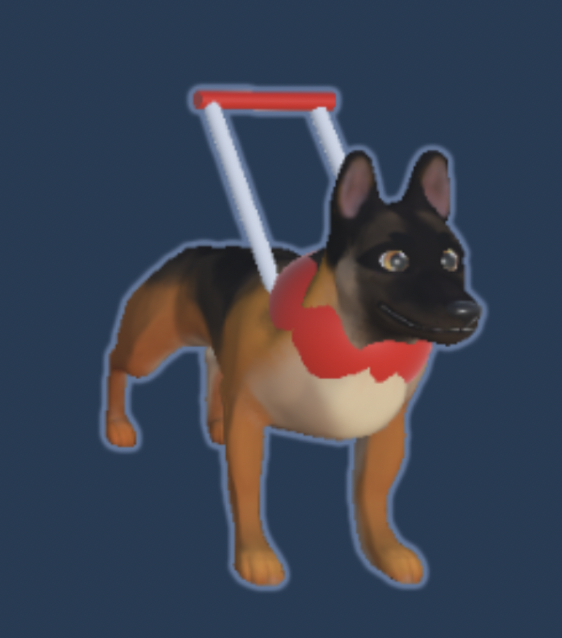
\includegraphics[width=2cm, height=2cm]{dog_guide.png}} & German-shepherd with black and brown fur, wearing a bright-red guide dog harness. & Walks beside the user on their left side. The sounds of panting and paws scratching the floor indicate movement. & \textit{Nova,} feminine voice, low formality (uses slang, jokes, and casual speech), averages 185.4 words per response & Very friendly, excited companion who is eager to please who you’re talking to & \textit{What an exciting world we're in! To your right stands the impressive Tall Building, reaching up high with its yellow facade…} \\
                    \hline
                    \textbf{Robot} & \raisebox{-\totalheight}{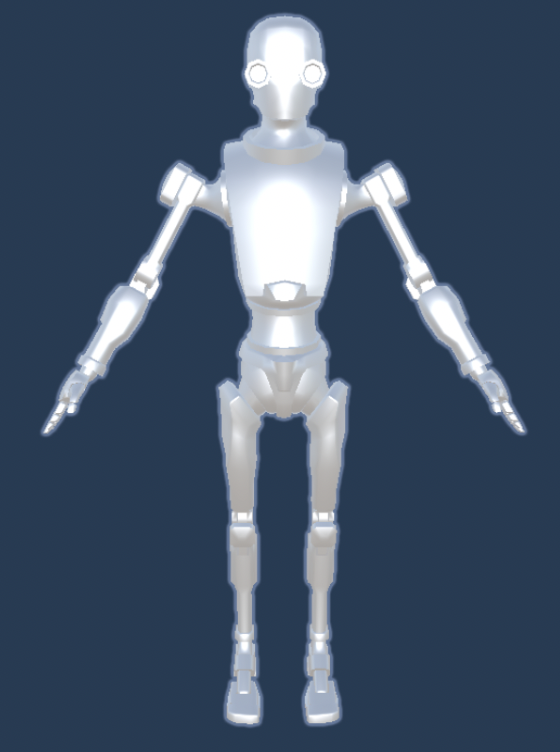
\includegraphics[width=1.8cm, height=2.3cm]{robot_guide.png}} & A shiny, silver robot that is humanoid in stature, with a masculine frame. & Follows behind the user from an arm’s length away. Creaking machinery sound effects indicate movement. & \textit{Onyx,} masculine voice, high formality (speaks entirely in proper sentences, no casual speech), averages 91.2 words per response & Formal and assertive assistant who talks like a robot & \textit{Affirmative. The area around you is composed of geometric shapes and structures. Directly to your right lies the Tall Building…} \\
                    \hline
                \end{tabular}
                \newline\newline
                \Description{Information about three different guide personas. Contains all textual content, aside from the three images of the persona's avatars in the column "Guide Avatar." Each avatar is described in the following column "Guide Description."}
            \end{center}
        \end{table*}

In our original work, we also proposed six guide “personas,” or combinations of different appearances and personalities, to provide varied guidance experiences. While a comprehensive evaluation of all personas is an area for future research, our objective was to evaluate the AI guide's core functionality, so we implemented only three within our refined guide: the dog, the robot, and the human (see Table \ref{tab: Guide Personas}). We selected the dog because it is a familiar physical-world guide form that also serves as a disability signifier. We chose the robot to be a fantastical form representative of the unique experiences possible in VR. Finally, we used the human for the tutorial, as its similarity to a human sighted guide facilitated an easier transition to the VR framework. We named all personas "Giddy," unlike the original AI guide which had no name. This decision—intended to give the guide a simple, short, and androgynous name—was based on suggestions from BLV participants in pilot studies informing our updated AI guide design.

To replicate the initial guidance experience from our human guide study, we re-utilized two virtual park environments from that study \cite{collins2023guide}. The first park had a calm environment with a square pathway and a river, while the second was more lively, featuring a complex pathway and a group of dancers. We also included a tutorial environment with simplistic objects for training purposes (see Figure \ref{fig: Virtual Environments}).

We implemented our VR prototype in Unity, following our original specifications from Collins et al. \cite{collins2024ai}. Navigation relied on Unity's NavMesh and NavAgents pathfinding components, and user queries were processed via OpenAI APIs. We used OpenAI's Speech-to-Text model, Whisper, to convert verbal queries to text, which was then sent to GPT-4 along with environment screenshots captured at the time of the query and hosted in a temporary image server. The guide then sorted these queries into five categories with different output types and used descriptors to embody the intended persona. To assess system responsiveness, we defined and recorded the guide's response time as the duration from the end of the user's speech input to the start of the guide's audio output. Finally, we built our prototype on a Meta Quest 2. Utilizing a visually-dominant VR headset presents a potential tradeoff of increasing cognitive load or physical discomfort for BLV users experiencing it as an audio-centric system. However, we chose this hardware to ensure the prototype's compatibility with standard, widely-available commercial VR ecosystems and consumer VR experiences.

Prior to deployment, we investigated several Speech-to-Text models for their robustness, including Google's Speech-to-Text API and Microsoft’s Azure AI Speech. We selected OpenAI’s Whisper due to its integration within the same API services as GPT-4 (also from OpenAI). This unified architecture allowed for more seamless data transfer between our STT and LLM endpoints, resulting in lower operational costs and lower end-to-end latency during pilot testing. Ultimately, Whisper performed adequately for our general population.

In addition to the basic prompt structure from our prior work, we developed a new prompt section based on pilot study feedback. This section instructed GPT-4 to write responses specifically for a blind user, incorporating best practices identified by our BLV pilot participants. These practices included using distances, cardinal directions, and references to the user's position relative to known objects. We also limited responses to 200 words or less to prevent overwhelming the user with extraneous detail, a limitation not imposed in our prior work. Finally, the guide was instructed to structure its responses directly to the user, as sometimes, it would reply as if to an unknown third party. The full prompt is available in our supplemental materials.

\subsection{Data and Analysis}
We collected video recordings of the VR tasks and audio recordings of the semi-structured interviews. Four researchers then transcribed and coded these recordings using a mixed-methods approach.

First, three researchers coded a transcript with closed codes to: (1) tally the number of participant-guide interactions and the guide’s correct responses, and (2) note types of interactions between the participant and guide, following interaction categorizations from our human guide study \cite{collins2023guide}. Discrepancies were discussed and a consensus reached before dividing remaining transcripts for coding. The closed codes were analyzed separately to complement the qualitative findings.

For the qualitative data, two researchers coded a transcript with open codes to create an initial codebook, which was then applied to the remaining transcripts. This was followed by an inductive thematic analysis \cite{clarke2017thematic, braun2019reflecting} using affinity diagramming to identify emerging themes.

As part of coding interactions, researchers needed to classify the tones in which participants addressed the guide. We initially used tone categories from our previous work with the human guide (utilitarian, friendly, respectful, apologetic, and uncertain) \cite{collins2023guide}. However, after finding no instances of behaviors like apologizing or deferring expertise, we reduced the categories to utilitarian, friendly, and polite. We reclassified "respectful" to "polite" based on coder consensus that participants were not offering consistent respect, but using occasional polite markers like "please" and "thank you." We classified any queries where participants used such phrases as “polite.”

To classify friendly and utilitarian speech, we deferred to external sources on social dynamics and linguistics. We defined “friendly” queries based on behaviors that foster social connection \cite{angelo2015, goodwin1990}. For example, studies on social dynamics note that using a person's name or offering greetings demonstrates friendliness or connection \cite{angelo2015, goodwin1990}. Thus, we classified queries where participants used the guide’s name, a nickname, or greeted the guide before asking questions as “friendly” interactions. Conversely, a “utilitarian” tone was defined by language that ordered the guide to perform actions without social markers. Following linguistic classifications of imperative language \cite{kaufmann2011}, we identified utilitarian queries by their sentence structures, which manifested as orders, commands, or requests with no polite or friendly alterations.